
\documentclass[10pt]{article}
\usepackage{graphicx}
\usepackage{amsmath}
\usepackage{amssymb}
\usepackage{amsthm}
\usepackage{amsthm} 

\newtheorem{hypothesis}{Hypothesis} 
\usepackage{pdflscape}
\usepackage{afterpage}
\usepackage{rotating}
\usepackage{color}
\usepackage{placeins}
%\usepackage{paralist}
\usepackage{graphicx}
%\usepackage[retainorgcmds]{IEEEtrantools}
%\usepackage{hyperref}
\usepackage{caption}
\usepackage{floatrow}
\floatsetup[table]{capposition=top}
\usepackage{subcaption}
\usepackage{booktabs}
\usepackage{tabularx}
\usepackage{multirow}
\newcolumntype{Y}{>{\centering\arraybackslash}X}
\usepackage{natbib}
 \usepackage{tikz}
 \usepackage{changes}
\usetikzlibrary{decorations.pathreplacing}
\usepackage{longtable}
\usepackage[flushleft]{threeparttable}
\usepackage{framed}
%\usepackage{soul}
\usepackage{subfiles}
\bibpunct{(}{)}{;}{a}{}{,}
\graphicspath{{./plot/}}
\usepackage{array}
\newcolumntype{H}{>{\setbox0=\hbox\bgroup}c<{\egroup}@{}}

\makeatletter
\newcommand*{\textoverline}[1]{$\overline{\hbox{#1}}\m@th$}
\makeatother

%%% PAGE DIMENSIONS
 %%% PAGE DIMENSIONS
 \usepackage[margin=1.5in]{geometry}
 \geometry{a4paper}
\usepackage{setspace}
\doublespacing

\title{Cultural Similarity and Team Performance: Evidence from Professional Doubles Tennis}
\author{}
\date{\today}

\begin{document}


\maketitle
\thispagestyle{empty}

\begin{abstract}

Cultural similarity may facilitate team formation and coordination, yet evidence of whether culturally similar teams produce superior team performance remains mixed. We examine this question using all men’s doubles matches in Grand Slams from 2018 to 2025.  Culturally similar teams are more likely to win matches. However, this association has a clear boundary: it disappears in tiebreaks, where competing teams are closely matched and the outcome is determined over a few points. The association is stronger as team members have accumulated more professional experience but remains muted as the experience gap between teammates widens. Finally, we provide evidence that while there is substantial cultural sorting in team formation, stronger individuals are not systematically more likely to select culturally similar partners, suggesting that our results are not purely driven by endogenous sorting among stronger players.

%we provide descriptive evidence around the Olympic cycles likewise does not support this explanation. 
\end{abstract}
\newpage
\section{Introduction}
Many forms of work increasingly give individuals substantial discretion over whom they collaborate with, including entrepreneurial co-founders choosing business partners, researchers choosing co-authors, consultants assembling project teams, and professionals such as physicians, surgeons, and lawyers forming small working teams. %In these settings, teams are not necessarily assembled entirely through managerial assignment: individuals often have a say in whom they work with, and collaboration is therefore partly the outcome of endogenous partner choice. 
Understanding how individuals form these partnerships is important because the characteristics that shape partner formation may subsequently affect how well collaborators work together.

As organizations and professional networks become increasingly international, these collaborations often bring together individuals from different national, linguistic, and cultural backgrounds. Among the many characteristics that may shape these choices, cultural similarity is one potentially important dimension of team formation process. Individuals may prefer culturally similar collaborators because shared language, norms, or backgrounds can facilitate communication, reduce coordination costs, and make it easier to anticipate one another's actions. %At the same time, cultural similarity may come at the expense of exposure to different perspectives and skills. 
Recent work from Békés and Ottaviano (2025) show that culturally similar players are more likely to pass to one another within elite football teams. %Yet whether cultural similarity between collaborators ultimately translates into better team performance, particularly when collaborators themselves have substantial discretion over partner selection, remains less clear.
This raises a more specific question: \lq\lq When individuals have substantial discretion over whom they collaborate with, does cultural similarity between the resulting collaborators translate into better performance?" 

Answering this question requires a setting in which partner formation and subsequent team performance can both be observed. Professional doubles tennis provides such a real world international setting. %This makes it possible to study cultural similarity at the collaborator-pair level while explicitly recognizing that the partnership itself is endogenous to partner choice. Using data on men’s doubles matches at the four Grand Slam tournaments from 2018 to 2025, we examine whether teams whose members share a nationality, share an official language, or have greater linguistic proximity are more likely to win their matches. Doubles tennis also offers an unusually transparent team-production environment: individual contributions during play are directly observable, limiting concerns about unobserved effort and free-riding that can complicate team-performance measures in other settings. The central challenge is therefore less whether players contribute effort than how effectively the two players coordinate those contributions.
Two individuals bilaterally form a partnership and jointly work in a transparent team-production environment: individual contributions during play are directly observable, limiting concerns about unobserved effort and free-riding that can complicate team-performance measures in other settings. Moreover, individuals operate under high-stake economic incentives to maximize joint success. 
%Doubles tennis has the same basic organizational structure at a much smaller scale: two interdependent individuals repeatedly make decisions whose value depends partly on anticipating and adapting to the partner's actions. Although these settings differ substantially in purpose and context, they share common organizational challenges. %team members must repeatedly coordinate their actions under time constraints while adapting to rapidly changing environments. 
%Doubles tennis captures these fundamental features in a particularly transparent way. Every point requires two teammates to coordinate positioning, movement, tactical decisions, and responses to their opponents, while success depends not only on individual ability but also on how effectively partners anticipate and complement each other's actions. At the same time, performance is measured objectively, tasks are standardized across teams, and teammates operate under strong economic incentives to maximize joint success. These characteristics make doubles tennis an informative empirical model of organizational coordination in environments where communication and mutual understanding are essential to team performance.


In this paper, we use professional men's doubles tennis as an empirical setup to examine 1) the relationship between cultural similarity and team performance, and 2) the extent to which cultural similarity reflects systematic partner sorting. We collect data from all men's doubles matches in Grand Slams between 2018 and 2025. We measure cultural similarity along three complementary dimensions: shared nationality, shared official language, and linguistic proximity. We first examine whether culturally similar teams are more likely to win their matches. We then use tiebreak outcomes to examine a theoretically important boundary condition: whether the association remains visible when the opportunity for teammates to coordinate is sharply compressed. Tiebreaks are played to decide a set once the score reaches 6--6. They are short and closely contested in which relatively few points determine the outcome and teammates have fewer opportunities to communicate and adjust during play.\footnote{Much like a penalty shootout in football, a tennis tiebreak breaks a draw by shifting the match into a rapid-fire point-by-point format where losing a point on your own serve is the psychological equivalent of missing a penalty kick, as the alternating sequence means a single miss often decides the entire set.}
%\added{Recent work also documents cultural sorting in team interactions. Békés and Ottaviano (2025), for example, show that culturally similar players are more likely to collaborate in professional football. We find a similar pattern in professional doubles tennis, where partnerships are substantially more likely to connect culturally similar players than would be expected under random matching. This naturally raises a second question: once partnerships are formed, does cultural similarity also translate into differences in team performance? We address this question first and subsequently return to partnership formation to examine how cultural sorting operates in our setting.}
We find that culturally similar teams are 3.6 to 4.6 percentage points more likely to win Grand Slam matches, with the strongest and most precisely estimated associations observed for the language-based measures. This association, however, has a clear boundary. Cultural similarity is not associated with tiebreak outcomes. Tiebreaks provide a particularly stringent setting in which to examine the performance relevance of coordination: the competing teams have already demonstrated closely matched performance, while the outcome is determined over a short sequence of points that provides relatively little time and opportunity for teammates to communicate, adjust, and coordinate. The potential benefits of cultural similarity may therefore be too small to become visible under these conditions. If culturally similar teams were simply stronger for some persistent reason unrelated to coordination, we would have some reason to expect their advantage to remain visible in tiebreaks. Instead, the association is present when performance is aggregated over the match but not when the outcome is determined over a short, closely contested sequence. We interpret this contrast as evidence of a boundary condition on when cultural similarity can be associated with team performance, rather than as evidence of a universal performance advantage.


%We collect data from all men's doubles matches in the Grand Slam tournaments between 2018 and 2025.  Cultural similarity is measured by shared nationality, shared official language, and linguistic proximity, respectively. These measures capture different aspects of common cultural and communicative background. We examine whether cultural similarity is associated with match outcomes as well as tiebreak outcomes. Tiebreaks are played to decide a set once the score reaches 6--6. They are short and closely contested in which relatively few points determine the outcome and teammates have fewer opportunities to communicate and adjust during play.\footnote{Much like a penalty shootout in football, a tennis tiebreak breaks a draw by shifting the match into a rapid-fire point-by-point format where losing a point on your own serve is the psychological equivalent of missing a penalty kick, as the alternating sequence means a single miss often decides the entire set.}

%We find that culturally similar teams are \textcolor{blue}{3.8 to 4.7 percentage points} more likely to win  matches. The association is statistically significant across all three measures of  cultural similarity, with the strongest and most precisely estimated associations for shared language and linguistic proximity. However, these associations disappear in tiebreaks.  This difference is consistent with cultural similarity being related to coordination processes that have greater scope to operate over the course of a full match than within a short, closely contested sequence, where communication opportunities are more limited and point-level variation plays a greater role in determining the outcome. 

We next conduct a specificity robustness check by examining whether the observed association between cultural similarity and match performance is robust across playing surfaces.\footnote{\added{Tennis Grand Slams are contested across three distinct structural profiles: grass at Wimbledon, clay at the French Open, and hardcourts at the Australian and US Opens. These surfaces fundamentally alter communication dynamics.}} The coefficients are similar and stable across all surfaces, providing no evidence that the results are driven by a particular playing surface. 


We then investigate two distinct roles of professional experience through which cultural similarity may be associated with team performance. %,both related to players’ professional experience. 
First, more experienced players have accumulated greater task-specific knowledge and familiarity with high-level competition. Shared language and cultural background may facilitate communication and help teammates integrate this knowledge into coordinated action. If so, the association between cultural similarity and performance should be stronger among teams with greater professional experience. Second, cultural similarity may facilitate knowledge transfer through communication between experienced and less experienced teammates. If so, the association should strengthen with the within-team experience gap. We find the association between cultural similarity and match performance becomes stronger with team average professional experience, but not more valuable when teammates differ more in experience, suggesting that cultural similarity complements accumulated professional experience in communication and coordination.

Finally, we return to the endogenous team formation stage. We document the extent of cultural sorting in partnerships, examine whether this sorting is particularly pronounced among stronger players. Cultural similarity is substantially more common among observed partnerships than under random matching, confirming that doubles teams are strongly sorted by nationality and language. However, this sorting is not more pronounced among higher-ranked players, and a player's own ranking is, if anything, negatively associated with having a culturally similar partner. We therefore find no evidence for the specific selection explanation in which stronger players systematically choose culturally similar partners. Nevertheless, these descriptive analyzes cannot rule out other forms of endogenous partner selection.

\added{TO LITERATURE: A large literature has examined the relationship between cultural composition and team performance, with mixed and context-dependent findings. In their meta-analysis of 108 studies covering more than 10,000 teams, Stahl et al. (2010) find that cultural diversity is associated with greater creativity but also greater conflict and lower social integration, with little overall effect on team performance. }

\added{A particularly relevant recent contribution is Békés and Ottaviano (2025), who show that cultural homophily remains pervasive in the interaction patterns of highly skilled professional football players, using passing behavior in Europe's top five men's leagues. Their evidence establishes that cultural similarity is associated with whom players interact with within multinational teams, even in settings characterized by high skill, common objectives, and strong incentives to cooperate. We take this pattern of culturally structured interaction as an important starting point and ask a complementary question: does cultural similarity also translate into differences in the ultimate performance of small teams? Rather than examining who interacts with whom within an established team, we study whether culturally similar partnerships are associated with superior team outcomes, and whether such an association persists when the opportunity for coordination to influence performance is sharply constrained. Békés and Ottaviano (2025) study cultural homophily in collaboration within professional football teams, where players operate within an organizational structure in which team composition and interaction opportunities are substantially shaped by managerial decisions. Our setting differs in an important respect: doubles partnerships are formed largely through bilateral decisions by individual players, with limited intervention from a manager or other central authority. This provides a setting in which cultural similarity can enter both the formation of partnerships and subsequent team performance.}

Our study relates to \added{three} strands of literature. First, it contributes to the literature on cultural diversity and organizational performance. Economic models emphasize the trade-off between diversity's informational benefits and its communication costs \citep{lazear1999}, while organizational research documents that cultural diversity simultaneously enhances creativity and knowledge variety but also creates coordination challenges and interpersonal conflict \citep{stahl2010,harrisonklein2007}. Although numerous studies examine workforce diversity and firm outcomes, relatively few identify the role of cultural similarity within small teams performing highly interdependent tasks.

Second, our paper contributes to the literature on language, communication, and organizational coordination. Language has been recognized as a fundamental organizational resource that facilitates information exchange, knowledge integration, and collective decision-making \citep{wernerfelt2004}. In international business and organizational research, language differences have been shown to impede knowledge transfer and collaboration across multinational organizations \citep{marschanpiekkari1999,feelyharzing2003}. Related evidence from economics shows that linguistic similarity reduces communication frictions and facilitates economic interaction, including trade, migration, and cross-border collaboration \citep[e.g.,][]{melitztoubal2014}. Our analysis extends this literature by examining whether shared language is associated with performance in teams whose success depends on continuous real-time coordination rather than one-off communication. \added{HERE}

Third, we relate to the literature on shared mental models and team coordination. Organizational researchers argue that high-performing teams develop common understandings of tasks and teammates that enable implicit coordination, particularly in environments characterized by repeated interaction and rapidly changing conditions \citep{cannonbowers1993,klimoski1994,mathieu2000}. While this literature has primarily relied on laboratory experiments and organizational settings, our study provides evidence from elite professional teams performing under naturally occurring competitive conditions, where coordination quality is reflected directly in objective performance outcomes.

%Finally, our paper builds on the emerging literature examining cultural homophily in professional sports. Most closely related is the recent  study by \citet{bekesottaviano2025}, which shows that professional football players exhibit systematic cultural homophily in passing behaviour, indicating that cultural similarity shapes patterns of collaboration even within highly professional organizations. Whereas that study focuses on who collaborates with whom, we examine whether cultural similarity is associated with how successfully teams perform once formed. By distinguishing collaboration from performance, we address a complementary question about the organizational consequences of cultural homophily.

This paper makes three important contributions. First, it extends the literature on cultural homophily from collaboration to objective team performance. Second, it identifies a boundary condition: the association disappears in short, closely contested tiebreaks, suggesting that cultural similarity matters most when teammates have sufficient opportunity for coordination advantages to accumulate. Third, it shows that the association between cultural similarity and performance becomes stronger with teammates' professional experience, consistent with coordination benefits developing through repeated interaction. 

The remainder of the paper is organized as follows. Section 2 describes the data, measures of cultural similarity, and construction of the empirical sample. Section 3 develops the theoretical framework and hypotheses. Section 4 presents the empirical analysis of cultural similarity and team performance. Section 5 investigates two potential mechanisms related to players’ professional experience. Section 6 returns to the formation of partnerships, documenting cultural sorting, examining whether stronger players are more likely to form culturally similar partnerships, and describing team formation around the Olympic cycles. Section 7 concludes.
\section{Data}
\subsection{Empirical Setting and Sample}
Our empirical setting consists of men's doubles matches from the four Grand Slam tournaments, the Australian Open, Roland Garros, Wimbledon, and the US Open, between 2018 and 2025. The dataset contains 1,864 completed Grand Slam doubles matches and $3{,}728$ team-match observations.\footnote{\textcolor{red}{From the initial dataset with 1,933 matches we first exclude 12 qualifying-round matches found only at Wimbledon 2018 (8 ``1st Round Qualifying'' and 4 ``2nd Round Qualifying'' matches present in the raw data but not part of the main draw at any other tournament-year -- a data-inclusion inconsistency, not a real difference in draw size), leaving 1,921 matches. We then exclude retirements and walkovers because these outcomes do not reflect normal competitive performance. We further remove matches with incomplete doubles ranking information that cannot be reliably recovered, resulting in a final sample of 1,864 matches.}}

Player information is collected by combining official tournament records from the Association of Tennis Professionals (ATP)  and supplementary public sources. Nationality and language information are fully harmonized through a multi-stage validation procedure that resolves inconsistencies arising from spelling variants, accented characters, and historical nationality changes. %Only observations for which all four players have complete ranking and cultural information are retained.


\begin{table}[htbp]
\color{blue}
\centering
\caption{Observation Breakdown and Descriptive Statistics}
\label{tab:t1}
\begin{threeparttable}
\textbf{Panel A: Matches by Tournament and Year (regression sample)}\\[2pt]
\textcolor{red}{
\begin{tabular}{lccccccccc}
\toprule
Tournament & 2018 & 2019 & 2020 & 2021 & 2022 & 2023 & 2024 & 2025 & \textbf{Total} \\
\midrule
Australian Open & 60 & 62 & 63 & 62 & 59 & 63 & 60 & 61 & \textbf{490} \\
Roland Garros    & 63 & 60 & 62 & 62 & 62 & 61 & 58 & 63 & \textbf{491} \\
Wimbledon        & 61 & 61 & 0  & 60 & 59 & 61 & 61 & 62 & \textbf{425} \\
US Open          & 63 & 60 & 31 & 59 & 62 & 61 & 63 & 59 & \textbf{458} \\
\midrule
\textbf{Total} & \textbf{247} & \textbf{243} & \textbf{156} & \textbf{243} & \textbf{242} & \textbf{246} & \textbf{242} & \textbf{245} & \textbf{1,864} \\
\bottomrule
\end{tabular}
}

\vspace{10pt}
\textbf{Panel B: Descriptive Statistics}\\[2pt]
\textcolor{red}{
\begin{tabular}{lcccc}
\toprule
 & \multicolumn{2}{c}{Individual level ($N$=7,456)} & \multicolumn{2}{c}{Team level ($N$=3,728)} \\
Variable & Mean & SD & Mean & SD \\
\midrule
Doubles ranking            & 126.02 & 210.46 & 126.02 & 183.51 \\
Years since turning pro    & 12.59  & 5.36   & 11.93  & 5.17   \\
Age at tournament          & 31.57  & 5.19   & 31.60  & 4.36   \\
Top-100 singles player (share) & \multicolumn{2}{c}{--} & \multicolumn{2}{c}{8.1\%} \\
\bottomrule
\end{tabular}
}
\begin{tablenotes}
\small
\item Note: Individual-level statistics pool both teammates across all 3,728 team-obs (4 players $\times$ 1,864 matches, minus a small number with missing tenure/DOB). Team-level statistics are the two-teammate average used directly in the regressions (\textit{rank\_mean}, \textit{exp\_mean}, \textit{age\_mean}). Years since turning pro is imputed to 1 for 216 team-obs whose raw tenure is $\le 0$ (rookies who turned pro in or after the tournament year); the team-level mean above reflects this imputation.
\end{tablenotes}
\end{threeparttable}
\end{table}
%\FloatBarrier

Table~\ref{tab:t1} reports the number of matches in each tournaments by year in Panel A and descriptive statistics at both individual and team level in Panel B. 


\subsection{Measuring Cultural Similarity}
We construct three  measures of cultural similarity. The first measure, Same Nationality, equals one if both teammates represent the same country and zero otherwise. The second measure, Same Language, equals one if both teammates share an official national language. The third measure, Language Proximity, is a continuous measure ranging from zero to one that captures the linguistic similarity between teammates' native languages, with larger values indicating greater linguistic proximity.

These measures reflect increasingly broad notions of cultural similarity. Shared nationality captures common institutional and cultural background. Shared language more directly captures communication potential. Linguistic proximity recognizes that communication costs may also be lower between speakers of closely related languages even when they do not share the same official language.



\begin{table}[htbp]
\color{blue}
\centering
\caption{Shares of the Three Cultural Similarity Measures, and Unique Teams by Tournament}
\label{tab:t2}
\begin{threeparttable}
\begin{tabular*}{\textwidth}{l@{\extracolsep{\fill}}l}
{\footnotesize
\begin{tabular}{lc}
\toprule
\multicolumn{2}{l}{\textbf{Panel A: Cultural Similarity Shares}} \\[2pt]
\toprule
Measure & Share \\
\midrule
Same nationality  & 42.2\% \\
Same language  & 56.0\% \\
Ling.\ proximity (0--1) & 0.568 \\
\bottomrule
\end{tabular}%
}
&
{\footnotesize
\begin{tabular}{lc}
\toprule
\multicolumn{2}{l}{\textbf{Panel B: Partnerships by Tournament}} \\[2pt]
\toprule
Tournament & Teams \\
\midrule
Australian Open & 542 \\
Roland Garros & 543 \\
Wimbledon & 487 \\
US Open & 517 \\
\midrule
\textbf{Total} & \textbf{2,089} \\
\bottomrule
\end{tabular}%
}
\end{tabular*}
\begin{tablenotes}
\small
\item Note: Panel A reports shares over the 2,089 distinct tournament$\times$partnership pairings with complete ranking data (same rank-complete sample as Panel B and Section~\ref{sec:sorting}'s Table~\ref{tab:t9} ``All'' row) -- a pair advancing through several rounds of the same event is counted once, not once per match played. Panel B counts the same 2,089 pairings, broken down by tournament.
\end{tablenotes}
\end{threeparttable}
\end{table}
\FloatBarrier

In our sample,  \textcolor{red}{42.2\%} of teams consist of players sharing the same nationality, \textcolor{red}{56.0\%} share an official language, and the mean linguistic proximity is \textcolor{red}{0.568} on the 0--1 scale.

\section{Theory and Hypotheses}
\subsection{Cultural Similarity and Team Performance}
A central concept in the organization literature is the idea of shared mental models. Teams develop shared representations of tasks, roles, priorities, and appropriate responses to different situations. When team members hold sufficiently similar understandings of these dimensions, they can anticipate one another's actions and coordinate without having to communicate every decision explicitly. Related work on implicit coordination emphasizes that effective teams can rely on shared expectations when responding to recurring situations. Transactive memory systems provide a complementary perspective: through repeated interaction, team members develop an understanding of what their teammates know and how knowledge and responsibilities are distributed within the team.

These perspectives suggest that coordination depends partly on reducing the cognitive and communication costs of joint action. Culture and language can affect these costs. Teammates who share a language may communicate intentions more easily and interpret verbal and non-verbal cues more consistently. Shared nationality may capture additional dimensions of cultural familiarity, including norms, expectations, and common social experiences. More generally, linguistic proximity may reduce communication barriers even when teammates do not share a nationality or an official language.

The implication is not that cultural similarity directly makes a team better. Rather, cultural similarity may make it easier for teammates to combine their individual abilities into effective joint performance. %This distinction is central to our analysis. We are interested in the coordination return to cultural similarity, rather than in differences in individual ability associated with nationality, language, or culture. 
We therefore propose:
\begin{hypothesis}
 Teams with greater cultural similarity are more like to win matches  than culturally dissimilar teams.
\end{hypothesis}
\subsection{Tiebreaks as a Boundary Condition}

\added{Tiebreaks impose a different temporal and competitive environment in which the opportunity for any coordination advantage to accumulate is substantially reduced.}

The coordination benefits associated with cultural similarity are not necessarily  equally observable in every part of a match. Coordination is a process that develops through repeated interaction: teammates communicate, adjust their behavior, learn one another's tendencies, and build shared expectations. While a full match provides a series of opportunities for this process to operate, a tiebreak substantially
compresses these opportunities.\footnote{Two distinct tiebreak formats exist in professional tennis. A \emph{standard} tiebreak, played to decide a set once the game score reaches 6--6, is won by the first team to reach 7 points with a margin of at least 2 (so it typically lasts 7--10 points in practice); this format is used in every set of a match, and, at some tournaments, in the final set as well. A \emph{match} or ``super'' tiebreak, played to 10 points instead of 7, is used at some tournaments as a substitute for a full final set. \added{In our sample, no genuine 10-point match tiebreak is ever used to decide the last set at any of the four Grand Slams. Wimbledon is the only tournament with a non-standard deciding-set format: in 15 of our sample's matches (7 in 2018, 3 in 2019, 5 in 2021), the last set was instead resolved through extended advantage-set play with no breaker at all, with final scores such as 16--14 and 22--20 -- consistent with Wimbledon's pre-2019 rule of no tiebreak in the deciding set and, for the 2019 and 2021 cases, with its subsequent 12-12-breaker rule simply never being triggered because the set ended before reaching 12-12. At the Australian Open, Roland Garros, and US Open -- and in the remaining 79 Wimbledon matches with a completed deciding set -- the last set is instead resolved by the same standard 6--6 seven-point breaker used in every other set.}} First, tiebreaks are short relative to the match as a whole, leaving less time for a coordination advantage to accumulate. Second, a tiebreak is reached only when the two teams have performed sufficiently similarly to reach a closely contested stage of the set. Its outcome is therefore determined in a setting where relatively small differences in performance can be decisive and where point-level randomness is likely to play a larger role.

%The communication environment also differs. During a set, teammates have repeated opportunities to communicate during changeovers, allowing them to exchange information, adjust tactics, and coordinate subsequent play. A tiebreak substantially compresses these opportunities. Once the tiebreak begins, teammates have very limited scope for formal discussion before the decisive points are played, with the principal changeover occurring only after the score reaches 6–6. Thus, a tiebreak provides not only a shorter horizon over which coordination can operate but also fewer opportunities to communicate and update a shared understanding during that period.

 These features make the tiebreak a particularly informative boundary condition. If cultural similarity improves team performance partly by facilitating communication in adjusting tactics and coordinating subsequent play, its advantage should be less apparent in a short, closely contested sequence in which there are fewer opportunities for communication and greater scope for point-level randomness. This leads to our second hypothesis:

\begin{hypothesis}
%The performance advantage associated with cultural similarity is weaker in tiebreaks than in overall match outcomes.
The positive association between cultural similarity and team performance is weaker when the opportunity for teammates to coordinate is limited, such as in short, closely contested episodes.
\end{hypothesis}

\section{Empirical Analysis}

\subsection{Match Performance}
\label{sec:matchwin}
We test Hypothesis 1 by  estimating the association between cultural similarity of the two players within a team and the probability of winning a doubles match. Specifically, we estimate a Logit model
\begin{equation}\label{matchoutcome}
  \operatorname{Pr}(W_{ijt} = 1) = f(\beta C_{ijt} + \gamma X_{ijt} + \delta_{ty} + \lambda_r) , 
\end{equation}


where $W_{ijt}$ equals one if team $i$ wins match $j$ in tournament-year $t$, $C$ denotes one of our three measures of cultural similarity: same nationality, same language, and language proximity. 
X includes three sets of control variables. First, observable own team and opponent team qualities, measured using the average ATP individual doubles ranking of each  players.\footnote{\added{The ATP does not publish a persistent, tournament-by-tournament doubles ranking at the pair level: the doubles rankings we scrape are strictly individual, one entry per player, with no team or pairing identifier. The only ATP ranking computed at the pair level is the season-only Doubles Race, used exclusively to seed qualification for the year-end ATP Finals; it resets every calendar year and is defined only for pairs that have accumulated enough joint results together that season, so it does not exist for a large share of our sample -- doubles partnerships change frequently across tournaments, and many Grand Slam pairings are new or infrequent. Each player's own individual ranking, by contrast, is continuously available regardless of current partner, so we use the two teammates' average individual ranking as the team-quality measure.}} Lower ranking values indicate stronger players. Second, an indicator for whether either teammate in own team is ranked inside the ATP Top 100 in singles, capturing exceptional individual talent that may not be reflected fully in doubles rankings. Third, professional experience measured as the average number of years since the two teammates turned professional. To allow for diminishing returns, we also include its squared term. 

Throughout the analysis we include tournament-by-year fixed effects $\delta_{ty}$ and round fixed effects $\lambda_r$ to absorb common variation across tournaments and stages of competition. Standard errors are clustered at the match level to account for interdependent team-match observations.





\begin{table}[htbp]
\color{blue}
\centering
\caption{Match Win — Average Marginal Effects (AME) from Logit \label{tab:t3}}
\begin{threeparttable}
\begin{tabular}{lccc}
\toprule
 & (1) Same Nationality & (2) Same Language & (3) Lang. Proximity \\
\midrule
Cultural similarity & 0.0361** & 0.0459*** & 0.0419*** \\
 & (0.0164) & (0.0157) & (0.0157) \\
Own avg. doubles ranking & $-$0.0007*** & $-$0.0007*** & $-$0.0007*** \\
 & (0.0001) & (0.0001) & (0.0001) \\
Opponent avg. doubles ranking & 0.0007*** & 0.0007*** & 0.0007*** \\
 & (0.0001) & (0.0001) & (0.0001) \\
Top-100 singles player (0,1)& $-$0.0042 & $-$0.0030 & $-$0.0024 \\
 & (0.0315) & (0.0315) & (0.0315) \\
Team avg. professional years  & 0.0044*** & 0.0043** & 0.0042** \\
 & (0.0017) & (0.0017) & (0.0017) \\
Team avg. professional years$^2$  & $-$0.0008*** & $-$0.0008*** & $-$0.0008*** \\
 & (0.0002) & (0.0002) & (0.0002) \\
\midrule
Tournament $\times$ year FE & Yes & Yes & Yes \\
Match round FE & Yes & Yes & Yes \\
Pseudo-$R^2$ & 0.096 & 0.097 & 0.097 \\
$N$ & 3,728 & 3,728 & 3,728 \\
\bottomrule
\end{tabular}
\begin{tablenotes}
\small
\item *** p$<$0.01, ** p$<$0.05, * p$<$0.10. Standard errors in parentheses, clustered by match. Unit of observation is team-match (2 team obs. per match); Professional years (Experience) is demeaned at the sample mean (11.93 years)
% ; the squared term is built from the demeaned variable. %so the linear term is the marginal effect of tenure at the sample mean.
\end{tablenotes}
\end{threeparttable}
\end{table}
\FloatBarrier

Table~\ref{tab:t3} reports average marginal effects (AMEs) estimated in logit models. %which can be interpreted as percentage-point changes in the probability of winning associated with each explanatory variable.
Across all three specifications, culturally similar teams are significantly more likely to win Grand Slam matches. The estimated effects range from 3.6 to 4.6 percentage points and are strongest when cultural similarity is measured through shared language. Team quality are the dominant predictor of success: stronger own doubles rankings significantly increase the probability of winning, while stronger opponent rankings significantly decrease the probability of winning. Whether having a top 100 singles player in the team does not seem to matter for the match outcome. More experienced teams perform better with diminishing returns.

\added{Alternative specification: randomly assign one team per match as the focal team to be kept in the regression analysis (N=1,864). Coefficients are of similar magnitude and slighter weaker significance.} \textcolor{red}{Repeated over 10 random seeds: the same-nationality AME averages 0.0466 (range 0.0161--0.0812, significant at the 5\% level in 5 of 10 draws), same-language averages 0.0517 (range 0.0230--0.0877, significant in 7 of 10 draws), and language proximity averages 0.0471 (range 0.0156--0.0859, significant in 6 of 10 draws). Similar to Table 3 but slightly different magnitude, as expected from halving the sample and inflating standard errors by roughly $\sqrt{2}$.}

These findings provide consistent evidence that cultural similarity is positively associated with team performance after accounting for observable differences in own and opponent quality,  experience, and tournament characteristics.

\subsection{Disentangling Nationality from Language}
\label{sec:natlang}
\added{The \textit{same\_country} and \textit{same\_language} measures used above are themselves correlated: in our sample, every same-nationality team-obs is also a same-language team-obs (0 team-obs share a nationality but not an official language), so Table~\ref{tab:t3} alone cannot distinguish whether the cultural-similarity association reflects shared nationality specifically -- e.g.\ shared sporting institutions, geographic proximity, or common exposure on the junior circuit -- or a broader communication-related component tied to language. To separate the two, we replace the two indicators with three mutually exclusive categories that partition the full estimation sample: (i) \textit{same nationality and same language}; (ii) \textit{different nationality, same language} (e.g.\ Germany/Austria, UK/Australia/US, Spain/Argentina -- teammates who share a language without sharing an institutional or geographic background); and (iii) \textit{different nationality, different language} (the omitted reference category). Table~\ref{tab:t4} reports the sample sizes, raw win rates, and re-estimated AMEs for these categories using the same controls, fixed effects, and clustering as Table~\ref{tab:t3}.}

\begin{table}[htbp]
\color{blue}
\centering
\caption{Match Win: Nationality vs.\ Language Decomposition \label{tab:t4}}
\begin{threeparttable}
\begin{tabular}{lccc}
\toprule
 & $N$ & Win rate & AME \\
\midrule
Same nationality + same language & 1,534 & 49.0\% & 0.0467*** \\
 & & & (0.0173) \\
Diff.\ nationality + same language & 561 & 56.9\% & 0.0438* \\
 & & & (0.0230) \\
Diff.\ nationality + diff.\ language (reference) & 1,633 & 48.6\% & -- \\
\midrule
Own avg. doubles ranking & & & $-$0.0007*** \\
 & & & (0.0001) \\
Opponent avg. doubles ranking & & & 0.0007*** \\
 & & & (0.0001) \\
Top-100 singles player (0,1) & & & $-$0.0031 \\
 & & & (0.0315) \\
Team avg. professional years & & & 0.0043** \\
 & & & (0.0017) \\
Team avg. professional years$^2$ & & & $-$0.0008*** \\
 & & & (0.0002) \\
\midrule
Tournament $\times$ year FE & \multicolumn{3}{c}{Yes} \\
Match round FE & \multicolumn{3}{c}{Yes} \\
Pseudo-$R^2$ & \multicolumn{3}{c}{0.097} \\
$N$ (total) & \multicolumn{3}{c}{3,728} \\
\bottomrule
\end{tabular}
\begin{tablenotes}
\small
\item *** p$<$0.01, ** p$<$0.05, * p$<$0.10. Standard errors in parentheses, clustered by match. Same controls and FE as Table~\ref{tab:t3}. Reference category (omitted): different nationality, different language. The three categories partition the full estimation sample exactly (0 same-nationality/different-language team-obs exist in this data).
\end{tablenotes}
\end{threeparttable}
\end{table}

\added{The key comparison is between the two same-language rows. Same-nationality teams (who are, by construction in this data, also same-language) show a positive and highly significant association with winning (AME = 0.0467, p$<$0.01). Critically, different-nationality teams who share a language show an association of similar magnitude (AME = 0.0438) that is significant at the 10\% level (p = 0.057), despite this being the smallest of the three groups (561 team-obs). Because these teammates share no nationality -- and therefore no shared sporting federation, junior-circuit exposure, or geographic proximity -- this result is inconsistent with the cultural-similarity association being driven solely by nationality-specific institutional factors. It is more consistent with a communication-related component of cultural similarity that operates through shared language independently of shared nationality.}

\subsection{Testing Tiebreaks as a Boundary Condition}
%Tiebreaks provide a particularly demanding boundary test because they are both short and conditional on the two teams having reached a closely contested state. The limited number of points leaves less scope for coordination advantages to accumulate, while the outcome of a short sequence is more sensitive to point-level variation.


%\begin{itemize}
%\item Compression: there are relatively few points over which coordination advantages can accumulate.
%\item Selection into a close contest: the tiebreak is reached when the two teams have been sufficiently evenly matched in that part of the match.
%\item Greater outcome variance: A short sequence of points is more susceptible to individual point-level events, so even if cultural similarity improves coordination, that advantage may be harder to detect in the winner of one tiebreak.
%\end{itemize}

The match-level results establish a positive association between cultural similarity and team performance. We next ask whether this association persists when the opportunity for team coordination is substantially compressed. This provides a boundary condition for the interpretation of the main results. If cultural similarity is associated with performance because shared cultural and communication backgrounds facilitate coordination between teammates, its performance relevance should depend partly on whether teammates have sufficient opportunity to communicate, adjust to one another, and anticipate one another's actions. The longer the task, the more opportunities teammates have to develop and apply such coordination. By contrast, a tiebreak is a short and highly compressed sequence in which relatively few points determine the outcome.

This setting is particularly informative because a tiebreak is played after the two teams have already demonstrated closely matched performance within the match. The outcome is therefore determined over a much shorter sequence than the match as a whole, leaving less time and opportunity for communication-related coordination advantages to accumulate. At the same time, point-level variation is likely to account for a larger share of the final outcome. Thus, even if cultural similarity is associated with better coordination over the course of a match, its potential performance benefits may be too small to become visible when the competing teams are sufficiently close in performance and the outcome is determined over only a small number of points.

We estimate the same specification used for the match-level analysis, replacing the match-win outcome with an indicator for winning the tiebreak. Table 4 reports the results. Across all three measures of cultural similarity, the estimated associations are substantially smaller than those observed for match outcomes and are not statistically distinguishable from zero. The absence of a detectable association is consistent across shared nationality, shared official language, and linguistic proximity.

The contrast between the two outcomes is informative. If culturally similar teams were simply stronger for some persistent reason unrelated to coordination, there would be less reason to expect their advantage to disappear precisely when the outcome is compressed into a short sequence. Instead, the association is visible when performance is aggregated over the course of the match but not when the outcome is determined over a brief, closely contested episode. We interpret this pattern as a boundary condition on the performance relevance of cultural similarity: potential coordination benefits may require sufficient time and opportunity to emerge and accumulate, and may therefore be difficult to detect when teams are closely matched and the task provides too little scope for teammates to communicate and adjust.

We estimate the same empirical specification in Equation (\ref{matchoutcome}) using tiebreak results as the outcome variable.


\begin{table}[htbp]
\color{blue}
\centering
\caption{Tiebreak Win — Average Marginal Effects (AME) from Logit \label{tab:t5}}
\begin{threeparttable}
\begin{tabular}{lccc}
\toprule
 & (1) Same Nationality & (2) Same Language & (3) Lang. Proximity \\
\midrule
Cultural similarity & 0.0308 & 0.0082 & 0.0026 \\
 & (0.0224) & (0.0218) & (0.0217) \\
Own avg. doubles ranking & $-$0.0003*** & $-$0.0003*** & $-$0.0003*** \\
 & (0.0001) & (0.0001) & (0.0001) \\
Opponent avg. doubles ranking & 0.0003*** & 0.0003*** & 0.0003*** \\
 & (0.0001) & (0.0001) & (0.0001) \\
Top-100 singles player (0,1) & $-$0.0675 & $-$0.0646 & $-$0.0644 \\
 & (0.0428) & (0.0427) & (0.0427) \\
Team avg. professional years & 0.0027 & 0.0023 & 0.0022 \\
 & (0.0022) & (0.0021) & (0.0021) \\
Team avg. professional years$^2$ & 0.0000 & 0.0001 & 0.0001 \\
 & (0.0003) & (0.0003) & (0.0003) \\
\midrule
Tournament $\times$ year FE & Yes & Yes & Yes \\
Round FE & Yes & Yes & Yes \\
Pseudo-$R^2$ & 0.013 & 0.013 & 0.013 \\
$N$ & 2,354 & 2,354 & 2,354 \\
\bottomrule
\end{tabular}
\begin{tablenotes}
\small
\item *** p$<$0.01, ** p$<$0.05, * p$<$0.10. Standard errors in parentheses, clustered by match. Unit of observation is team-tiebreak (2 team obs. per tiebreak); standard 7-point tiebreaks only. Same controls and FE as Table \ref{tab:t3}.
\end{tablenotes}
\end{threeparttable}
\end{table}
\FloatBarrier

Table \ref{tab:t5} reports the results. None of the three measures of cultural similarity is significantly associated with the probability of winning a tiebreak. The estimated coefficients are economically small and statistically indistinguishable from zero.  The ranking controls remain highly significant, indicating that the specification continues to capture underlying differences in team quality.

\added{If culturally similar teams were simply stronger for some persistent reason, we would have some reason to expect that advantage to remain visible in tiebreaks.}

Taken together, these findings suggest that the association between cultural similarity and team performance has an important condition: it is more likely to emerge when teammates have sufficient opportunity to coordinate over the course of a task. The positive association with match outcomes, combined with its absence in tiebreaks, is consistent with cultural similarity mattering through coordination processes that can accumulate over time, rather than providing an advantage that operates equally in every episode of team performance. If culturally similar teams were simply stronger for some persistent reason, we would expect that advantage to remain visible in tiebreaks. Instead, the association is present when performance is aggregated over the match but not when the outcome is determined over a short, closely contested sequence. Tiebreaks therefore provide a particularly stringent boundary condition: when two teams are already performing very similarly, the potential performance benefit of cultural similarity may be too small to become visible over a short sequence, in which teammates have limited time and opportunity to communicate, adjust to one another, and translate coordination advantages into the final outcome.


\subsection{Robustness check: Testing Tennis-Specific Explanations} 


One concern is that the observed association reflects strategic characteristics unique to particular playing surfaces rather than general coordination processes. \added{Tennis Grand Slams are contested across three distinct structural profiles: grass at Wimbledon, clay at the French Open, and hardcourts at the Australian and US Opens. These surfaces fundamentally alter ball dynamics, where clay generates high friction that slows the ball and increases bounce height, grass minimizes friction to produce low, rapid trajectories, and hardcourts offer a standardized, intermediate speed and bounce. Consequently, these physical variances dictate distinct communication styles. On fast surface like grass, the rapid pace compresses decision-making windows, forcing partners to rely on pre-packaged tactical scripts and implicit, non-verbal cues because there is no time for mid-rally adjustments. Conversely, on slow surface like clay, longer rallies allow for active, asynchronous verbal feedback during the point, as well as more frequent emotional regulation and strategic recalibration between points to sustain high cognitive load.} 

If the observed association were driven by a particular tactical or environmental feature of doubles tennis, we might expect the return to cultural similarity to vary across surfaces, which differ substantially in their playing characteristics. We therefore test whether the association is stable across surfaces by interacting each cultural similarity measure with grass and clay surface, respectively. 


Table \ref{tab:t6} reports the results. The coefficients are remarkably stable across playing environments, suggesting that the result is not driven by any specific physical environment of the tournament \footnote{\textcolor{red}{As a robustness check, restoring tournament$\times$year FE and estimating C$\times$grass/C$\times$clay jointly (hardcourt as baseline, no separate surface main effect) leaves this conclusion unchanged: both C$\times$grass and C$\times$clay interactions remain small and insignificant (p$>$0.65) in that specification.}}. \textcolor{red}{The notes below every table (Tables \ref{tab:t3}--\ref{tab:t9}) have been checked against the underlying estimation code -- controls, fixed effects, clustering, sample sizes, and robustness-spec descriptions all match what was actually estimated.}


\begin{table}[htbp]
\color{blue}
\centering
\caption{Stability across playing surfaces \label{tab:t6}}
\begin{threeparttable}
\begin{tabular}{lcccccc}
\toprule
 & \multicolumn{2}{c}{(1) Same Nationality} & \multicolumn{2}{c}{(2) Same Language} & \multicolumn{2}{c}{(3) Lang. Proximity} \\
 & (a) grass & (b) clay & (a) grass & (b) clay & (a) grass & (b) clay \\
\midrule
Cultural similarity (C) & 0.0395** & 0.0351* & 0.0439** & 0.0477*** & 0.0416** & 0.0401** \\
 & (0.0183) & (0.0189) & (0.0176) & (0.0182) & (0.0176) & (0.0181) \\
Surface & 0.0097 & $-$0.0017 & $-$0.0022 & 0.0047 & 0.0019 & $-$0.0037 \\
 & (0.0149) & (0.0142) & (0.0207) & (0.0188) & (0.0209) & (0.0194) \\
C $\times$ Surface & $-$0.0169 & 0.0023 & 0.0070 & $-$0.0084 & 0.0003 & 0.0061 \\
 & (0.0376) & (0.0347) & (0.0364) & (0.0340) & (0.0364) & (0.0344) \\
\midrule
Controls  & Yes & Yes & Yes & Yes & Yes & Yes \\
Round FE & Yes & Yes & Yes & Yes & Yes & Yes \\
Tournament $\times$ year FE & No & No & No & No & No & No \\
Pseudo-$R^2$ & 0.096 & 0.096 & 0.097 & 0.097 & 0.096 & 0.096 \\
$N$ & \multicolumn{2}{c}{3,728} & \multicolumn{2}{c}{3,728} & \multicolumn{2}{c}{3,728} \\
\bottomrule
\end{tabular}
\begin{tablenotes}
\small
\item *** p$<$0.01, ** p$<$0.05, * p$<$0.10. Standard errors in parentheses, clustered by match. Spec (a): grass vs.\ rest (hardcourt+clay pooled). Spec (b): clay vs.\ rest (hardcourt+grass pooled). Round FE only; Same controls as in  Table \ref{tab:t3}. 
\end{tablenotes}
\end{threeparttable}
\end{table}
\FloatBarrier


\section{Roles of Professional Experience}

In this section we examine the roles of players’ professional experience which could shed light on potential mechanisms. Since our data do not directly observe communication or coordination processes, these analyses should be interpreted as mechanism-related heterogeneity tests rather than direct tests of the mechanisms themselves. %We focus on players’ professional experience and distinguish between two roles that experience could play. 

%First, greater professional experience may mean that teammates bring more task-relevant knowledge to the partnership. If cultural similarity facilitates the communication and integration of this knowledge, the association between cultural similarity and performance should increase with team average professional experience.


%Second, cultural similarity may facilitate knowledge transfer between teammates with different levels of professional experience. If so, its association with performance should become stronger as the experience gap within the team increases.

First, players with more years of professional experience are likely to have accumulated greater task-specific knowledge and a better understanding of the demands of high-level competition. When teammates share a language or broader cultural background, communication may make it easier to convey and integrate this experience into joint decision-making, allowing culturally similar teams to translate their individual professional knowledge into coordinated action more effectively. If this channel is important, the association between cultural similarity and performance should be stronger among teams whose members have greater professional experience. 

Second, cultural similarity may facilitate knowledge transfer when teammates differ substantially in professional experience. A shared language and cultural background may reduce communication barriers and make it easier for a more experienced player to communicate task-relevant knowledge to a less experienced partner. Under this interpretation, the association between cultural similarity and performance should become stronger as the experience gap within the team increases. %\added{But could it be that an unbalanced experience profile is a disadvantage in the first place? Cultural similarity may not be powerful enough to close the gap?}

%To sum, we first test whether cultural similarity is more strongly associated with performance when players have accumulated more individual professional experience. Then, we test whether cultural similarity becomes stronger as the experience gap within the team widens.

%—for example, by facilitating communication or knowledge transfer from the more experienced player to the less experienced one.

%In this section we investigate two distinct mechanisms through which cultural similarity may be associated with team performance, both related to players’ professional experience. First, players with more years of professional experience are likely to have accumulated greater task-specific knowledge and a better understanding of the demands of high-level competition. When teammates share a language or broader cultural background, communication may make it easier to convey and integrate this experience into joint decision-making, allowing culturally similar teams to translate their individual professional knowledge into coordinated action more effectively. If this channel is important, the association between cultural similarity and performance should be stronger among teams whose members have greater professional experience. Second, cultural similarity may facilitate knowledge transfer when teammates differ substantially in professional experience. A shared language and cultural background may reduce communication barriers and make it easier for a more experienced player to communicate task-relevant knowledge to a less experienced partner. Under this interpretation, the association between cultural similarity and performance should become stronger as the experience gap within the team increases. We find that the association between shared language and linguistic proximity and match performance becomes stronger with team average years since turning professional. In contrast, we find no evidence that cultural similarity is particularly valuable when teammates differ more in professional experience. The evidence is therefore more consistent with cultural similarity complementing the use of players’ accumulated professional knowledge in coordination than with a knowledge-transfer mechanism specifically arising from differences in experience.


%We examine two distinct mechanisms through which cultural similarity could be related to coordination. The first concerns accumulated professional experience: more experienced teammates may have developed greater ability to anticipate one another's actions and communicate efficiently, allowing cultural and linguistic similarity to become more valuable as professional experience accumulates. The second concerns within-team experience differences: cultural and linguistic similarity may instead be particularly valuable when teammates differ substantially in experience, because a common cultural and linguistic background could facilitate the transfer of knowledge and expectations from a more experienced player to a less experienced teammate. These mechanisms make different predictions. The first implies that the association between cultural similarity and performance should strengthen with the team's average professional experience; the second implies that it should strengthen with the experience gap between teammates.
\subsection{Average Professional Experience} 


%On the one hand, experienced professionals have developed richer tactical knowledge and communication routines, allowing them to exploit shared language more effectively. 
%\begin{itemize}
%\item Does cultural similarity become more valuable as teams accumulate experience? 
%\end{itemize}








We first test whether the association between cultural similarity and match performance varies with team average experience. For each team, we calculate the average number of years since the two players turned professional. \added{Notice that this is not the years the two players have been working together in the same team, but the average individual professional experience of the two players.}\footnote{\added{In tennis, partnership can change relatively often. Players may team up with different partners in different tournaments. Calculate how many teams and the share in total have repeated partnership during the sample period and how many unique team appearance.}} We interact this measure with cultural-similarity while retaining the full set of controls and fixed effects from the baseline specification in Equation (\ref{matchoutcome}). That is, we estimate the following model
\begin{equation}
\operatorname{Pr}(\text{Win}) = f(\beta_1 C + \beta_2 \text{AvgTeamExp} + \beta_3 (C \times \text{AvgTeamExp}) + \gamma X + \delta_{ty} + \lambda_r)
\end{equation}

%Team average experience is demeaned at its sample mean of 11.93 years, so the coefficient on cultural similarity represents its association with match performance for a team at the average level of professional experience. The specification also includes the linear and quadratic terms for average experience used in the main analysis.

Table \ref{tab:t7} reports the results. The interaction between cultural similarity and team average experience is positive for all three measures. For same nationality, however, the interaction is very small and statistically insignificant (0.0008, p=0.809). For the two language-based measures, the interaction is positive and statistically significant: 0.0069 for shared language (p=0.032) and 0.0068 for linguistic proximity (p=0.034). Thus, the association between language-related cultural similarity and match performance becomes stronger as team members have more professional experience on average.


\begin{table}[htbp]
\color{blue}
\centering
\caption{Team Average Experience \label{tab:t7}}
\begin{threeparttable}
\begin{tabular}{lccc}
\toprule
 & (1) Same Nationality & (2) Same Language & (3) Lang. Proximity \\
\midrule
Cultural similarity (C)  & 0.0361** & 0.0433*** & 0.0392** \\
 & (0.0164) & (0.0157) & (0.0156) \\
C $\times$ exp\_mean\_dm & 0.0008 & 0.0069** & 0.0068** \\
 & (0.0033) & (0.0032) & (0.0032) \\
exp\_mean\_dm (main) & 0.0041* & 0.0002 & 0.0002 \\
 & (0.0023) & (0.0025) & (0.0025) \\
\midrule
Controls & Yes & Yes & Yes \\
Tournament $\times$ year FE & Yes & Yes & Yes \\
Round FE & Yes & Yes & Yes \\
Pseudo-$R^2$ & 0.096 & 0.098 & 0.097 \\
$N$ & 3,728 & 3,728 & 3,728 \\
\bottomrule
\end{tabular}
\begin{tablenotes}
\small
\item *** p$<$0.01, ** p$<$0.05, * p$<$0.10. Standard errors in parentheses, clustered by match. \textit{exp\_mean\_dm} is demeaned at the sample mean (11.93 years, SD 5.17), so the Culture (C) row is the AME at mean team experience.
\end{tablenotes}
\end{threeparttable}
\end{table}
\FloatBarrier



The result is robust to allowing the interaction to vary nonlinearly with experience. When we additionally include the interaction between cultural similarity and squared demeaned experience, the quadratic interactions are small and statistically insignificant for all three measures (p$>$0.50), while the linear interactions for shared language and linguistic proximity remain positive and statistically significant. %The finding therefore does not appear to be driven by an omitted nonlinear relationship.

This pattern is consistent with a mechanism based on accumulated professional experience and the development of effective coordination. More experienced players may be more able to anticipate teammates' actions and establish efficient communication routines. Cultural and linguistic similarity may make these coordination processes more effective, so that their association with performance becomes stronger among more experienced teams. The fact that the result is concentrated in the language-based measures is particularly consistent with a communication-based interpretation.

Importantly, our measure captures players' individual professional experience, rather than the number of matches a particular pair has played together. We therefore do not directly observe the development of pair-specific shared mental models or communication routines. The evidence should consequently be interpreted as consistent with, rather than establishing, a process in which professional experience strengthens the performance relevance of cultural and linguistic similarity.


\subsection{Experience Gaps within the Team} 

On the other hand, shared language becomes especially valuable when teammates differ substantially in expertise because communication and knowledge transfer become more demanding. Large experience gaps imply asymmetric knowledge, asymmetric decision authority, coaching/mentoring,
 and more need to transfer tacit knowledge. That is exactly where shared language may matter most. \added{The experience-gap analysis asks whether cultural similarity is particularly valuable when teammates differ in professional experience, conditional on the team's overall competitive strength and average professional experience. That is, among teams with comparable overall strength and comparable average professional experience, does cultural similarity become particularly valuable when the two teammates differ more in professional experience?}

The estimating equation becomes
\begin{align}
\operatorname{Pr}(\text{Win}) = f(\beta_1 C + \beta_2 \text{TeamExpGap} + \beta_3 (C \times \text{TeamExpGap}) + \gamma X + \delta_{ty} + \lambda_r)
\end{align}
%There may be greater uncertainty about: how the less experienced player behaves; tactical preferences; positioning; risk-taking; communication; expectations about the partner. Shared language could potentially reduce those coordination frictions.




The second mechanism makes a different prediction. Cultural similarity may matter particularly when teammates have different levels of professional experience. An experienced player may possess greater knowledge of the demands of elite doubles competition, while an inexperienced teammate may need to learn unfamiliar routines and expectations. Under this knowledge-transfer interpretation, a common cultural and linguistic background could facilitate communication between teammates with different levels of experience. The value of cultural similarity should therefore increase with the experience gap within the team, rather than with the average experience of the two players.

We test this prediction using the absolute difference between the two teammates' years since turning professional, ExperienceGap=. We interact this measure with each cultural-similarity measure and additionally control for team average experience and its quadratic term. The experience gap is demeaned at its sample mean of 5.50 years, so the cultural-similarity coefficient is evaluated at the average experience gap rather than at zero. The models otherwise retain the specification used in the main analysis.


\begin{table}[htbp]
\color{blue}
\centering
\caption{Within-Team Experience Gap \label{tab:t8}}
\begin{threeparttable}
\begin{tabular}{lccc}
\toprule
 & (1) Same Nationality & (2) Same Language & (3) Lang. Proximity \\
\midrule
Culture (C) -- mean gap & 0.0356** & 0.0447*** & 0.0409*** \\
 & (0.0164) & (0.0157) & (0.0157) \\
C $\times$ exp\_gap\_dm & 0.0032 & 0.0038 & 0.0036 \\
 & (0.0034) & (0.0032) & (0.0032) \\
exp\_gap\_dm (main) & $-$0.0036* & $-$0.0045* & $-$0.0045* \\
 & (0.0021) & (0.0025) & (0.0025) \\
\midrule
Controls (Table~\ref{tab:t3} set) & Yes & Yes & Yes \\
Tournament $\times$ year FE & Yes & Yes & Yes \\
Round FE & Yes & Yes & Yes \\
Pseudo-$R^2$ & 0.097 & 0.097 & 0.097 \\
$N$ & 3,728 & 3,728 & 3,728 \\
\bottomrule
\end{tabular}
\begin{tablenotes}
\small
\item *** p$<$0.01, ** p$<$0.05, * p$<$0.10. Standard errors in parentheses, clustered by match. \textit{exp\_gap\_dm} $=|{\rm exp}_i-{\rm exp}_j|$, demeaned at the sample mean (5.50 years, SD 4.92); individual tenure is imputed to 1 year for rookies. Controls include team-average \textit{exp\_mean\_dm} and its square, plus \textit{exp\_gap\_dm} itself. A robustness spec adding C $\times$ exp\_gap\_dm$^2$ leaves the conclusion unchanged (quadratic term and linear term both insignificant throughout, p$>$0.29).
\end{tablenotes}
\end{threeparttable}
\end{table}
\FloatBarrier

The results provide no evidence that cultural similarity becomes more strongly associated with performance as the experience gap increases. The interaction is positive for all three measures—0.0032 for same nationality (p=0.344), 0.0038 for same language (p=0.232), and 0.0036 for linguistic proximity (p=0.261)—but none is statistically significant. Allowing for a quadratic relationship between the experience gap and cultural similarity produces the same conclusion: the quadratic interactions are small and statistically insignificant, while the linear interactions remain insignificant.

The results therefore distinguish the two potential mechanisms. We find evidence that the association between cultural similarity and performance becomes stronger among more experienced teams, particularly for language-related measures, but no evidence supporting the specific prediction that cultural similarity is especially valuable as a bridge across unequal experience levels. The findings are consequently more consistent with an interpretation based on accumulated professional experience and coordination.

This distinction is important for interpreting the mechanism. We do not find evidence that cultural similarity primarily helps an experienced player transmit knowledge to a less experienced teammate. Instead, the results point toward a setting in which the value of cultural and linguistic compatibility is greater among teams whose members have accumulated more professional experience. While this pattern is consistent with the gradual development of shared expectations and coordination routines, the available data do not allow us to observe those processes directly.



\section{Team Formation and Cultural Sorting}
An important feature of doubles tennis is that teams are formed bilaterally between players rather than assigned exogenously. This makes partnership formation relevant for interpreting the performance associations documented above. Békés and Ottaviano (2025) show that cultural similarity is systematically related to interaction patterns within professional football teams, demonstrating that culturally structured collaboration persists even among highly skilled professionals working in common organizational settings. Our data reveal a related pattern at the stage of team formation: players are substantially more likely to form partnerships with culturally similar teammates than would be expected under random matching. We therefore examine partnership formation separately from the performance analysis. The purpose of this section is not to eliminate selection concerns or to establish that partnerships are formed exogenously, but to document how cultural sorting operates in the doubles environment and whether it is particularly pronounced among stronger players. We first compare observed cultural similarity in partnerships with the corresponding random-matching benchmark, then examine whether a player's own doubles ranking predicts the cultural similarity of their partner, and finally describe how partnership formation varies around the Olympic cycles. Together, these analyses provide a more transparent picture of the selection environment in which the performance associations arise.

\subsection{Cultural Sorting in Partnership Formation}
\label{sec:sorting}


We construct a partnership-level sample containing each distinct men's doubles partnership appearing in the Grand Slams between 2018 and 2025. A partnership is counted once within a tournament, even if the same pair advances through several rounds, because partner formation occurs before the subsequent match outcomes. The resulting sample contains 2,089 partnerships with complete ranking information (542 at the Australian Open, 543 at Roland Garros, 487 at Wimbledon, and 517 at the US Open; see Table~\ref{tab:t2}, Panel B).

We compare the observed prevalence of cultural similarity with the rate expected under random matching within each tournament-year. The random-matching benchmark is calculated directly from the composition of the actual player field: for each tournament-year, we calculate the share of all possible player pairs that would satisfy the relevant cultural criterion. This produces a deterministic benchmark that accounts for the nationality and language composition of each tournament field.

\begin{table}[htbp]
\color{blue}
\centering
\caption{Cultural Sorting in Partnership Formation: Actual vs.\ Random-Matching Benchmark \label{tab:t9}}
\begin{threeparttable}
\begin{tabularx}{\textwidth}{l l Y Y Y}
\toprule
Measure & & All ranked players & Both partners top-100 & Both partners top-50 \\
 & & ($N$=2,089) & ($N$=1,211) & ($N$=712) \\
\midrule
\multirow{2}{*}{Same nationality} & Actual & 42.2\% & 32.6\% & 35.5\% \\
 & Random benchmark & 5.2\% & 4.1\% & 4.5\% \\
\multirow{2}{*}{Same language} & Actual & 56.0\% & 49.7\% & 56.3\% \\
 & Random benchmark & 16.2\% & 15.5\% & 15.8\% \\
\multirow{2}{*}{Mean ling.\ prox.} & Actual & 0.568 & 0.506 & 0.565 \\
 & Random benchmark & 0.199 & 0.189 & 0.189 \\
\bottomrule
\end{tabularx}
\begin{tablenotes}
\small
\item Note: one row per distinct partnership per tournament (2,089 partnerships, Grand Slams 2018--2025, Olympics excluded). Random benchmark is the closed-form expected rate under random pairing within each tournament-year's actual field, using the same CEPII \textit{comlang\_off}/\textit{comlang\_ethno} country-pair lookup underlying \textit{same\_language}/\textit{ling\_prox}.
\end{tablenotes}
\end{threeparttable}
\end{table}

The results in Table~\ref{tab:t9} show substantial cultural sorting. Among all partnerships, 42.2\% consist of players of the same nationality, compared with 5.2\% under random matching. Similarly, 56.0\% of partnerships share an official language, compared with 16.2\% under random matching. Mean linguistic proximity is 0.568 among observed partnerships, compared with 0.199 under random matching. Thus, doubles partnerships are strongly assortative along all three dimensions of cultural similarity.

This finding is important for interpreting the performance results. Cultural similarity is clearly not randomly distributed across partnerships: players who form teams are much more culturally similar than would be expected from the composition of the tournament field alone. The match-performance estimates should therefore not be interpreted as if cultural similarity were randomly assigned. Rather, they describe an association between the cultural composition of an already formed partnership and its subsequent performance.

At the same time, the sorting does not appear to be concentrated among the strongest players. Among partnerships in which both players are ranked in the top 100, 32.6\% are same-nationality partnerships, compared with 4.1\% under random matching. Among partnerships with both players in the top 50, the corresponding figures are 35.5\% and 4.5\%. The corresponding actual-to-random ratios are therefore remarkably similar across groups. The same pattern is evident for shared language and linguistic proximity. Indeed, the raw prevalence of same-nationality partnerships is lower among top-50 and top-100 partnerships than in the full sample, while same-language sorting remains broadly similar.

These comparisons provide no evidence that the cultural sorting observed in doubles is disproportionately driven by the strongest players.

\subsection{Player Ranking and Partner Selection}

We next examine the relationship between a player's own ranking and the cultural similarity of the partnership more directly. For each partnership, we treat each player in turn as the focal player, generating two player-level observations per partnership. This produces 4,178 player-partnership observations from the 2,089 partnerships. Because the same partnership contributes two observations, standard errors are clustered at the partnership level.

We regress each cultural-similarity measure on the focal player's own doubles ranking, including tournament-by-year fixed effects. \added{Because the cultural composition of the player pool differs across tournament-years, a player's probability of having a culturally similar partner may vary mechanically with the set of players entering the event. We therefore extend the specification to also account for the cultural composition of the tournament field: for each focal player, the share of every \emph{other} player in that tournament-year's full field (every entrant, not only the rank-complete partnerships used above) who shares the focal player's nationality -- and, analogously, the mean pairwise value of \textit{same\_language}/\textit{ling\_prox} against every other player in the field -- matched to the corresponding outcome.} The specification is deliberately parsimonious: the purpose is not to explain partner selection comprehensively, but to test whether a player's own ranking predicts the cultural similarity of the partner within a given tournament-year, and whether that association survives controlling for field composition.

The results are reported in Table~\ref{tab:t10}. In Spec 1 (own ranking alone), the coefficient on own ranking is positive and statistically significant for all three measures: 0.000269 for same nationality (p<0.001), 0.000146 for same language (p=0.012), and 0.000139 for linguistic proximity (p=0.009). Because a lower doubles-ranking number indicates a stronger player, the positive coefficient means that worse-ranked players are, if anything, more likely to have culturally similar partners.

\added{We estimate three specifications: (1) own ranking alone (as above); (2) the outcome-matched field-composition variable alone; and (3) own ranking plus field composition. All three specifications exclude the 3 ego-rows whose own nationality is represented by exactly one player in the ego-row sample, so that a single lone-nationality observation cannot by itself drive any coefficient; this leaves $N=4{,}175$ (from 4,178) throughout. We also estimated an own-nationality (country fixed effects) specification in place of own ranking, but do not report it: nationality is a 60-level categorical variable, so it produces 59 separate country-dummy coefficients rather than one interpretable effect, and its logit specifications fail to converge for the two binary outcomes regardless (quasi-complete separation, since several nationalities have as few as 2 ego-rows).}

\begin{table}[htbp]
\color{blue}
\centering
\caption{Own Ranking, Tournament-Field Composition, and Partner-Culture Similarity \label{tab:t10}}
\begin{threeparttable}
\begin{tabular}{lcccc}
\toprule
Outcome & Spec 1: & Spec 2: & Spec 3: & Spec 3: \\
 & own\_rank & composition & own\_rank & composition \\
\midrule
Same nationality (AME) & 0.000269*** & 3.853*** & 0.000116** & 3.756*** \\
 & (0.000056) & (0.241325) & (0.000053) & (0.255403) \\
Same language (AME) & 0.000146** & 1.275*** & 0.000117** & 1.267*** \\
 & (0.000058) & (0.081709) & (0.000053) & (0.082578) \\
Ling.\ proximity (OLS coef.) & 0.000139*** & 1.152*** & 0.000104** & 1.145*** \\
 & (0.000053) & (0.075655) & (0.000047) & (0.076295) \\
\midrule
$N$ (ego-rows) & 4,175 & 4,175 & 4,175 & 4,175 \\
\bottomrule
\end{tabular}
\begin{tablenotes}
\small
\item *** p$<$0.01, ** p$<$0.05, * p$<$0.10. Standard errors in parentheses, clustered by partnership. All specifications include tournament$\times$year FE and exclude ego-rows whose own nationality has exactly 1 observation in the ego-row sample (3 rows dropped; $N=4{,}175$, from 4,178). Field composition is (\# other field entrants sharing the focal player's nationality)/(field size $-1$) for same nationality, and the analogous mean pairwise value for same language / linguistic proximity, computed against every other player entering that tournament-year (not only the rank-complete partnerships in the estimation sample).
\end{tablenotes}
\end{threeparttable}
\end{table}

\added{Field composition alone (Spec 2) is also a strong, highly significant predictor of all three outcomes, as expected -- a player drawn from a tournament field with more compatriots or linguistically similar entrants is mechanically more likely to end up with a culturally similar partner. Adding both own ranking and field composition together (Spec 3) shrinks the own-ranking coefficients by roughly half relative to Spec 1 but leaves them positive and statistically significant for all three outcomes (p$<$0.05 throughout), while the composition coefficient stays close to its Spec 2 magnitude. Own ranking therefore predicts partner similarity \emph{in addition to}, not merely \emph{because of}, the cultural composition of the field a player happens to be drawn from.}

This result is the opposite of what would be expected if the performance association were primarily generated by stronger players having greater partner choice and systematically selecting culturally similar teammates. Together with the bracket comparisons, the evidence therefore provides no support for the specific selection mechanism in which stronger players disproportionately sort into culturally similar partnerships. It does not, however, eliminate other forms of endogenous partnership formation, and the performance estimates remain associations rather than causal effects.

\subsection{Team Formation Around the Olympic Cycle}
\added{The regular professional doubles circuit provides a setting in which players have substantial discretion over their partners, while Olympic doubles imposes a distinct institutional constraint: teams must represent the same nation. This raises a broader question about how institutional constraints interact with decentralized partnership formation. The Olympic requirement could, in principle, also increase the salience of national affiliation in the regular professional circuit, particularly as the Games approach, potentially generating spillovers in the cultural composition of Grand Slam partnerships.}

Finally, we provide a  descriptive perspective on partnership formation by examining whether cultural sorting changes around the Olympic Games. The Olympic Games provide a separate setting in which the incentives surrounding partner formation are particularly salient. Unlike Grand Slam doubles competition, Olympic participation is organized around national representation, creating a direct incentive for players seeking to compete together at the Games to form partnerships with compatriots. We therefore examine whether the composition of Grand Slam partnerships changes during the preparation periods surrounding the Tokyo 2021 and Paris 2024 Olympic Games. The analysis is descriptive and is intended to provide additional evidence on how partnership formation responds to the institutional environment surrounding elite competition.

For the Tokyo cycle, we divide the Grand Slam sample into three periods: a pre-Tokyo period covering the Australian Open 2018 through the US Open 2019; a Tokyo preparation period covering the Australian Open 2020 through Wimbledon 2021, excluding the cancelled 2020 Wimbledon; and a post-Tokyo period covering the US Open 2021 through the US Open 2022. For the Paris cycle, the pre-Paris period covers the 2022 Grand Slams, the Paris preparation period covers the Australian Open 2023 through Wimbledon 2024, and the post-Paris period covers the US Open 2024 through the US Open 2025.

\begin{table}[htbp]
\color{blue}
\centering
\caption{Grand Slam Partnerships Around the Tokyo 2021 and Paris 2024 Olympic Cycles \label{tab:t2ab}}
\begin{threeparttable}
\begin{tabular}{lcccccc}
\toprule
& \multicolumn{3}{c}{Tokyo 2021 cycle} & \multicolumn{3}{c}{Paris 2024 cycle} \\
\cmidrule(lr){2-4}\cmidrule(lr){5-7}
Measure & Pre-Tokyo & Tokyo Prep & Post-Tokyo & Pre-Paris & Paris Prep & Post-Paris \\
\midrule
Same nationality & 40.0\% & 40.3\% & 39.0\% & 39.3\% & 42.6\% & 43.9\% \\
Same language & 54.8\% & 55.0\% & 54.8\% & 54.1\% & 57.6\% & 58.8\% \\
Ling.\ proximity (mean) & 0.557 & 0.551 & 0.556 & 0.552 & 0.580 & 0.602 \\
\midrule
$N$ & 980 & 680 & 602 & 484 & 860 & 626 \\
\bottomrule
\end{tabular}
\begin{tablenotes}
\small
\item Note: Olympics excluded throughout. Windows: Pre-Tokyo = Jan 2018--Dec 2019; Tokyo Prep = Jan 2020--Jul 2021 (excludes Wimbledon 2020, cancelled); Post-Tokyo = Aug 2021--Dec 2022; Pre-Paris = Jan--Dec 2022; Paris Prep = Jan 2023--Jul 2024; Post-Paris = Aug 2024--Dec 2025.
\end{tablenotes}
\end{threeparttable}
\end{table}

The share of same-nationality teams is remarkably stable across the Tokyo cycle's three periods, at 40.0\%, 40.3\%, and 39.0\%, respectively (Table~\ref{tab:t2ab}). The corresponding shares for shared official language are 54.8\%, 55.0\%, and 54.8\%, while mean linguistic proximity is 0.557, 0.551, and 0.556.

The absence of an increase during the Tokyo preparation period is noteworthy because the Tokyo cycle took place during the COVID-19 pandemic. International travel and cross-border interaction were unusually difficult during this period, potentially increasing the relative attractiveness of partnering with compatriots or players from nearby linguistic communities. Nevertheless, the descriptive composition of teams does not show an increase in same-nationality or language-based partnerships during the preparation period.

\begin{figure}[htbp]
\centering
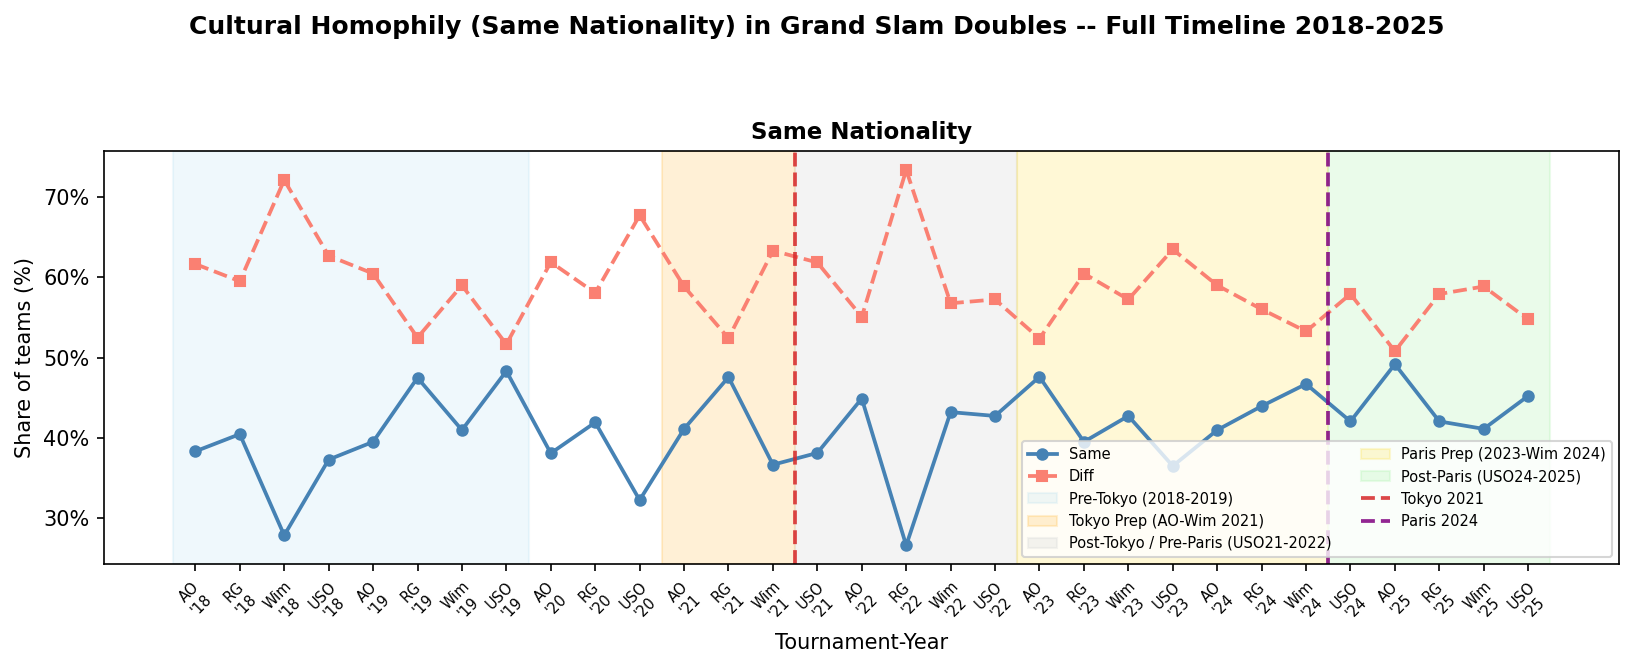
\includegraphics[width=\textwidth]{homophily_nationality_only}
\caption{Share of Grand Slam doubles teams sharing a nationality, 2018--2025, spanning both the Tokyo 2021 and Paris 2024 Olympic cycles. Shaded bands mark the pre/preparation/post periods used in Table~\ref{tab:t2ab}; dashed vertical lines mark the Games themselves.}
\label{fig:cycle_nat}
\end{figure}

The Paris cycle provides a contrasting pattern (Table~\ref{tab:t2ab} and Figure~\ref{fig:cycle_nat}). Same-nationality partnerships account for 39.3\% of teams before the Paris Games, 42.6\% during the preparation period, and 43.9\% afterwards. Shared-language partnerships increase from 54.1\% to 57.6\% and then 58.8\%, while mean linguistic proximity rises from 0.552 to 0.580 and then 0.602.

The contrast between the two Olympic cycles should not be interpreted as a causal estimate of Olympic incentives on partner formation. The two periods differ in many dimensions, most importantly the extraordinary conditions surrounding the Tokyo Games. Instead, the descriptive evidence illustrates that the composition of doubles partnerships can vary with the broader institutional and competitive environment. It also reinforces the broader conclusion from this section: partnership formation involves substantial cultural sorting, but that sorting is not simply a consequence of the strongest players systematically selecting culturally similar teammates.

\added{This evidence should be interpreted cautiously. The Olympics involve a small and highly selected set of players, and their qualification rules differ substantially from those governing the Grand Slam circuit. Moreover, the timing and strength of any spillover from Olympic participation or national representation to regular partnership decisions are not clear. Players may also respond to Olympic considerations in lower-level tournaments or through partnership decisions that are not captured by changes in the aggregate Grand Slam composition. We therefore do not interpret the stable pattern as evidence that the Olympic institution has no effect on partnership formation. Rather, it provides descriptive evidence that the heightened salience of national representation around the Olympics is not accompanied by a large, readily visible change in the cultural composition of the broader Grand Slam partnership market.}

Overall, the evidence in this section provides useful context for interpreting the main performance results. Cultural sorting is clearly present, but the data do not support the specific hypothesis that stronger players are disproportionately responsible for that sorting. At the same time, partnerships are formed through a mixture of deliberate choice and circumstances that can constrain partner selection. We therefore do not interpret the main estimates as causal effects of cultural similarity. Rather, the team-formation evidence helps assess the plausibility of one important alternative explanation for the observed association between cultural similarity and team performance.

%Taken together, the partnership-formation evidence provides two useful qualifications to the performance analysis. First, cultural sorting in doubles is substantial: culturally similar partnerships are much more common than random matching would imply. Second, the sorting does not appear to be disproportionately concentrated among higher-ranked players, and the Tokyo preparation period provides no evidence of a sharp increase in national sorting despite unusually strong incentives for nationally aligned preparation. These findings do not eliminate selection as a possible source of the performance association, but they make the specific explanation that stronger players systematically select culturally similar partners less consistent with the data.

\iffalse
\subsection{Evidence from the Olympics}

If cultural similarity is associated with better performance, an important question is whether players appear to sort toward culturally similar partners when the incentives to coordinate are particularly salient. We therefore examine team composition around the Tokyo and Paris Olympic cycles.  

\textcolor{red}{Table X reports the composition of teams across Olympic preparation cycles.} Despite widespread speculation that Olympic eligibility may encourage players to form same-nationality partnerships, the share of same-nationality teams remains remarkably stable during the Tokyo Olympic cycle. The Tokyo preparation period coincides with the covid period. During that period, international travel and international interaction were unusually constrained.

If anything, this creates a plausible setting in which same-nationality partnering could have been especially attractive: easier travel; fewer international logistical complications; greater opportunities to train together; potentially greater value from existing social/professional networks. Even in a period when practical constraints may have made same-nationality partnering particularly convenient, we do not observe an increase in same-nationality team formation.


During the Paris cycle, same-nationality and same-language partnerships become modestly more common, although the increase occurs gradually rather than as a discrete shift during the Olympic preparation period. These patterns do not provide evidence of systematic optimization.
\fi

\section{Conclusion}

\added{Attention: tennis doubles are formed by individual players, not by a manager or an organization. Different implications if were assigned by managers/organizations like football. The findings also have implications for organizations in which employees have discretion over their collaborators. In such settings, team composition may emerge partly through endogenous cultural sorting rather than solely through managerial assignment. If cultural similarity facilitates coordination, such sorting may reflect an economically meaningful feature of decentralized team formation. At the same time, our results do not imply that managers should systematically favor culturally similar teams: the evidence is observational, and culturally homogeneous partnerships may also reflect selection into partnerships on unobserved characteristics.}

Cultural diversity is increasingly a feature of how organizations assemble teams, but the organizational value of diversity depends not only on what individuals bring to a team but also on how effectively they can combine those resources. %This paper highlights one component of that process: the coordination costs associated with cultural differences. 
Our findings suggests that cultural similarity is associated with better team performance, but that this association is neither universal nor mechanical. Its relevance appears to depend on whether teammates have sufficient opportunity to communicate, develop shared understandings, and translate those understandings into coordinated action.

This perspective complements the recent finding that cultural homophily shapes collaboration even among highly skilled professionals in multinational football teams (Békés and Ottaviano, 2025). Their evidence shows that cultural similarity affects how teammates interact; our evidence suggests that such differences in interaction can also be reflected in collective performance. The distinction is important for management research. If cultural similarity matters partly because it lowers coordination costs, then its organizational consequences should depend on the structure of the task. Teams performing highly interdependent work, working under substantial time pressure, or relying on repeated interaction may be particularly sensitive to these costs. Conversely, organizations may be able to capture the informational benefits of cultural diversity when tasks allow greater time for communication, clearer division of responsibilities, or other mechanisms that reduce the need for implicit coordination.

\added{The performance relevance of cultural similarity depends on whether the structure of the task allows communication and coordination advantages to accumulate.}

The findings also suggest a more nuanced view of team composition. A natural managerial response to evidence of coordination costs would be to favor culturally similar employees when assembling teams. Our results do not justify such a prescription. Cultural similarity is strongly associated with partnership formation, but the evidence does not indicate that the strongest players are disproportionately responsible for this sorting. More importantly, our analysis is observational and cannot establish that cultural similarity itself causes superior performance. Cultural similarity may proxy for other dimensions of compatibility, partnership history, social networks, or unobserved characteristics that influence both team formation and performance. The evidence on experience is consistent with a role for accumulated shared experience, but it does not identify the precise process through which communication advantages develop.

\added{Cultural similarity may be more valuable when teams perform tasks requiring repeated interdependent coordination, communication, and adaptation. The value may be less visible when tasks are sufficiently short, tightly constrained, or dominated by small differences in performance. Managers should think about cultural composition jointly with task structure, rather than treating cultural similarity as inherently good or bad.Our evidence suggests that its performance relevance depends on whether team members have sufficient opportunity to communicate, adjust, and coordinate their actions over the course of a task.}

These limitations point toward an important agenda for future research. The central challenge is to move from observing cultural similarity to identifying the coordination process through which similarity affects team production. Experimental or quasi-experimental variation in team composition could help separate cultural compatibility from selection into partnerships. Richer longitudinal data could distinguish shared experience with a particular teammate from general professional experience and examine whether coordination routines develop through repeated interaction. Direct measures of communication—such as verbal exchanges, shared decision-making, or behavioral measures of anticipation—could provide an even more direct test of whether cultural and linguistic similarity operate through communication costs and shared mental models.

More broadly, the paper suggests that the consequences of diversity should be understood as a property of the interaction between team composition and task design, rather than as an inherent feature of diversity itself. Cultural differences may provide organizations with access to heterogeneous knowledge, perspectives, and networks, while simultaneously increasing the effort required to integrate those resources. Whether the balance is favorable depends on the extent to which an organization's production process relies on rapid, repeated, and interdependent coordination. Understanding this interaction is important for managers designing teams, but also for economists and organizational scholars seeking to explain when diversity becomes an asset, when it becomes a coordination challenge, and how organizations can reduce the costs of bringing different people together.

\appendix
\renewcommand{\thetable}{A\arabic{table}}
\setcounter{table}{0}
\section{Appendix: Robustness to Age as an Alternative Career-Maturity Proxy}
\color{red}
\textit{age\_mean} (team average player age at the tournament) is a second natural proxy for career maturity alongside \textit{exp\_mean} (years since turning pro); the two are highly correlated (corr = 0.83, implied VIF $\approx$ 3.32 if entered together), so age is estimated in its own separate specification rather than added alongside experience in the main tables.
\color{black}

\begin{table}[htbp]
\color{red}
\centering
\caption{Match Win, \textit{age\_mean} Replacing \textit{exp\_mean} \label{tab:ta1}}
\begin{threeparttable}
\begin{tabular}{lccc}
\toprule
 & (1) Same Nationality & (2) Same Language & (3) Lang. Proximity \\
\midrule
Cultural similarity & 0.0332** & 0.0447*** & 0.0409*** \\
 & (0.0164) & (0.0158) & (0.0157) \\
Own avg. doubles ranking & $-$0.0007*** & $-$0.0007*** & $-$0.0007*** \\
 & (0.0001) & (0.0001) & (0.0001) \\
Opponent avg. doubles ranking & 0.0007*** & 0.0007*** & 0.0007*** \\
 & (0.0001) & (0.0001) & (0.0001) \\
Top-100 singles player & 0.0077 & 0.0086 & 0.0089 \\
 & (0.0313) & (0.0313) & (0.0313) \\
Team avg. age at tournament & 0.0053** & 0.0052** & 0.0051** \\
 & (0.0023) & (0.0023) & (0.0023) \\
Age, squared & $-$0.0005 & $-$0.0006 & $-$0.0005 \\
\midrule
Tournament $\times$ year FE & Yes & Yes & Yes \\
Round FE & Yes & Yes & Yes \\
Pseudo-$R^2$ & 0.094 & 0.095 & 0.094 \\
$N$ & 3,728 & 3,728 & 3,728 \\
\bottomrule
\end{tabular}
\begin{tablenotes}
\small
\item *** p$<$0.01, ** p$<$0.05. Same sample, FE, and clustering as Table \ref{tab:t3}. Cultural-similarity AMEs are essentially unchanged from Table \ref{tab:t3} (e.g.\ same nationality: 0.0361 $\to$ 0.0332, both p$<$0.05), confirming the core finding is not an artefact of which career-maturity proxy is used.
\end{tablenotes}
\end{threeparttable}
\end{table}

\begin{table}[htbp]
\color{red}
\centering
\caption{Match Win, \textit{age\_mean} and \textit{exp\_mean} Entered Jointly (Diagnostic) \label{tab:ta2}}
\begin{threeparttable}
\begin{tabular}{lccc}
\toprule
 & (1) Same Nationality & (2) Same Language & (3) Lang. Proximity \\
\midrule
Cultural similarity & 0.0376** & 0.0467*** & 0.0425*** \\
Own avg. doubles ranking & $-$0.0007*** & $-$0.0007*** & $-$0.0007*** \\
 & (0.0001) & (0.0001) & (0.0001) \\
Opponent avg. doubles ranking & 0.0007*** & 0.0007*** & 0.0007*** \\
 & (0.0001) & (0.0001) & (0.0001) \\
Top-100 singles player & $-$0.0025 & $-$0.0014 & $-$0.0009 \\
 & (0.0315) & (0.0316) & (0.0316) \\
Team avg.\ yrs since turning pro & 0.0028 & 0.0027 & 0.0028 \\
 & (0.0029) & (0.0029) & (0.0029) \\
Yrs since turning pro, squared & $-$0.0008*** & $-$0.0008*** & $-$0.0008*** \\
Team avg.\ age at tournament & 0.0026 & 0.0025 & 0.0022 \\
 & (0.0040) & (0.0040) & (0.0040) \\
Age, squared & 0.0001 & 0.0001 & 0.0001 \\
\midrule
$N$ & 3,728 & 3,728 & 3,728 \\
\bottomrule
\end{tabular}
\begin{tablenotes}
\small
\item Diagnostic only, not a preferred spec. With both tenure proxies in the model, neither linear term remains significant (p$>$0.33), and SEs roughly double relative to the single-proxy specs -- the expected signature of near-collinear regressors (corr = 0.83), not evidence that career maturity stops mattering. The cultural-similarity AMEs remain robust throughout.
\end{tablenotes}
\end{threeparttable}
\end{table}

\begin{table}[htbp]
\color{red}
\centering
\caption{Tiebreak Win, \textit{age\_mean} Replacing \textit{exp\_mean} \label{tab:ta3}}
\begin{threeparttable}
\begin{tabular}{lccc}
\toprule
 & (1) Same Nationality & (2) Same Language & (3) Lang. Proximity \\
\midrule
Cultural similarity & 0.0253 & 0.0043 & $-$0.0013 \\
 & (0.0227) & (0.0221) & (0.0219) \\
Own avg. doubles ranking & $-$0.0003*** & $-$0.0003*** & $-$0.0003*** \\
 & (0.0001) & (0.0001) & (0.0001) \\
Opponent avg. doubles ranking & 0.0003*** & 0.0003*** & 0.0003*** \\
 & (0.0001) & (0.0001) & (0.0001) \\
Top-100 singles player & $-$0.0691 & $-$0.0672 & $-$0.0671 \\
 & (0.0428) & (0.0428) & (0.0427) \\
Team avg.\ age at tournament & $-$0.0002 & $-$0.0009 & $-$0.0010 \\
 & (0.0030) & (0.0030) & (0.0030) \\
Age, squared & 0.0002 & 0.0002 & 0.0002 \\
\midrule
Tournament $\times$ year FE & Yes & Yes & Yes \\
Round FE & Yes & Yes & Yes \\
Pseudo-$R^2$ & 0.013 & 0.012 & 0.012 \\
$N$ & 2,354 & 2,354 & 2,354 \\
\bottomrule
\end{tabular}
\begin{tablenotes}
\small
\item Same tiebreak sample, FE, and clustering as Table \ref{tab:t5}. As with experience, age is not significantly associated with tiebreak win (p$>$0.6 throughout), and none of the three cultural-similarity measures reach significance either -- the null tiebreak result is not an artefact of which career-maturity proxy is used.
\end{tablenotes}
\end{threeparttable}
\end{table}

\section{Appendix: Heterogeneity by Cultural Individualism (Hofstede IDV)}
\color{red}
As a further heterogeneity test, we interact each culture measure with the team-average Hofstede individualism score (\textit{IC\_team\_dm}, demeaned; mean = 62.98, SD = 20.85), testing whether teams from more individualist cultures rely less on in-group cultural bonding, so that the culture-performance association would be smaller for them.
\color{black}

\begin{table}[htbp]
\color{red}
\centering
\caption{Heterogeneity: Culture $\times$ Hofstede Individualism (Demeaned) \label{tab:ta4}}
\begin{threeparttable}
\begin{tabular}{lccc}
\toprule
 & (1) Same Nationality & (2) Same Language & (3) Lang. Proximity \\
\midrule
Culture (C) & 0.0293* & 0.0393** & 0.0352** \\
 & (0.0167) & (0.0163) & (0.0163) \\
IC\_team\_dm & 0.0011* & 0.0007 & 0.0007 \\
 & (0.0006) & (0.0008) & (0.0008) \\
C $\times$ IC\_team\_dm ($\theta$) & $-$0.00046 & 0.00007 & 0.00009 \\
 & (0.00079) & (0.00089) & (0.00089) \\
\midrule
Tournament $\times$ year FE & Yes & Yes & Yes \\
Round FE & Yes & Yes & Yes \\
Pseudo-$R^2$ & 0.097 & 0.098 & 0.097 \\
$N$ & 3,728 & 3,728 & 3,728 \\
\bottomrule
\end{tabular}
\begin{tablenotes}
\small
\item *** p$<$0.01, ** p$<$0.05, * p$<$0.10. Standard errors in parentheses, clustered by match. Hofstede IDV scores are taken from the official 6-dimension dataset (2015 release); countries not directly covered are assigned tiered proxy scores (direct cultural/linguistic kin, or same-region closest available). The interaction $\theta$ is small and statistically insignificant for all three measures (p$>$0.56), providing no evidence that individualism moderates the cultural homophily advantage. A robustness spec dropping team-obs relying on the lower-confidence regional proxy countries ($N=3{,}577$) leaves this conclusion unchanged.
\end{tablenotes}
\end{threeparttable}
\end{table}

\section{Appendix: Robustness to Non-Independence of Team-Rows within a Match}
\color{red}
Each match (tiebreak) contributes two team-rows that are mechanically linked -- a win for one team is a loss for the other -- so the two rows are not independent draws. The main specifications already address this via standard errors clustered by \textit{match\_id}. We verify this further with two checks. First, a no-intercept specification that gives tournament$\times$year fixed effects full-rank (all-levels) dummies instead of the usual intercept plus reference-dropped dummies reproduces Tables~\ref{tab:t3} and \ref{tab:t5} exactly (identical AMEs, SEs, and log-likelihood to three decimals), confirming it is a pure reparameterization rather than a different model. Second, we re-estimate both outcomes keeping only one randomly-selected team's row per match (Table~\ref{tab:t3}) or per tiebreak (Table~\ref{tab:t5}), removing the mechanical complementarity entirely; repeated over 10 random seeds since any single draw is arbitrary (the match-win version is reported in Section~\ref{sec:matchwin} above; the tiebreak-win version is reported here).
\color{black}

\begin{table}[htbp]
\color{red}
\centering
\caption{Robustness: One Randomly-Selected Team per Tiebreak (10 Random Seeds) \label{tab:ta5}}
\begin{threeparttable}
\begin{tabular}{lccc}
\toprule
Cultural similarity & Baseline AME & Random-one: mean AME [range] & Sig.\ ($p<.05$) \\
\midrule
Same nationality & 0.0308 (n.s.) & 0.0174~[$-$0.0305, 0.0592] & 1/10 \\
Same language & 0.0082 (n.s.) & $-$0.0041~[$-$0.0434, 0.0526] & 0/10 \\
Lang.\ proximity & 0.0026 (n.s.) & $-$0.0107~[$-$0.0526, 0.0433] & 0/10 \\
\bottomrule
\end{tabular}
\begin{tablenotes}
\small
\item Tiebreak win, $N\approx$1,177 per draw; all 10 seeds converge in every spec. Every point estimate keeps the same sign or a similarly small magnitude to baseline (Table \ref{tab:t5}), and none reaches significance -- consistent with the null tiebreak result. The stacked-both-rows, match-clustered design used throughout the paper remains the preferred specification.
\end{tablenotes}
\end{threeparttable}
\end{table}

\bibliographystyle{apalike}
\bibliography{reference}

\end{document}
